\documentclass[conference]{IEEEtran}

\usepackage{cite}
\usepackage{amsmath,amssymb}
\usepackage{newtxtext,newtxmath}
\usepackage{graphicx}
\usepackage{textcomp}
\usepackage{xcolor}
\usepackage{booktabs}
\usepackage{array}
\usepackage{tabularx}
\usepackage{url}
\usepackage[hidelinks]{hyperref}
\usepackage{microtype}

\graphicspath{{paper/figures/}}
\Urlmuskip=0mu plus 1mu
\newcolumntype{Y}{>{\raggedright\arraybackslash}X}
\newcommand{\Bench}{\textsc{MonopolyBench}}
\newcommand{\runid}[1]{\nolinkurl{#1}}

\begin{document}

\title{MonopolyBench: Auditing Long-Horizon Economic Agency in Multi-Agent Language Models}

\author{\IEEEauthorblockN{Anonymous Authors}}

\maketitle

\begin{abstract}
When long-running language-model agents are summarized primarily by terminal
task success, the resulting score can obscure how locally valid decisions
accumulate into durable advantage, fragility, or failure. We introduce
\Bench, an audit-ready
environment for studying long-horizon economic agency in a four-player
asset-and-solvency game. The authoritative rules engine alone generates
legal-action menus, mutates state, and emits events; language models select
among those actions, communicate, and emit model-authored private analysis
fields. The
resulting evidence contract links every provider attempt to its engine
decision, validation result, applied action, event range, state checkpoints,
communication, usage and cost when reported, and replay record. We distinguish
deterministic replay of engine transitions from stochastic regeneration of
model behavior, and separately test state replay and strict artifact replay.

We audit the instrument on eight completed games comprising 1,391 playable
turns, 3,696 engine decisions, and 3,790 provider attempts. All eight pass state
replay; seven pass strict artifact replay. The remaining run preserves every
applied action and the complete state trajectory but differs in two response
events' fallback-validity provenance. Evidence-indexed case studies recover mechanisms
hidden by win labels, including conversion of fragmented ownership into
developed rent engines, blocker-for-liquidity exchanges, finite-house
constraints, creditor-transfer compounding, and serialization failures at
solvency decisions. Because seats, rosters, model versions, seeds, and other
run conditions are unbalanced, the games constitute a mechanism corpus rather than a
leaderboard. \Bench\ contributes an enforceable economic decision surface and
a claim discipline for connecting outcomes to inspectable behavior,
reliability, and recorded resource use.
\end{abstract}

\begin{IEEEkeywords}
language-model agents, multi-agent systems, economic games, long-horizon
evaluation, negotiation, replay, provenance
\end{IEEEkeywords}

\section{Introduction}
\label{sec:introduction}

Language models increasingly act through sequences of state-changing
decisions rather than isolated answers. They call tools, negotiate with other
actors, allocate resources, and continue from states created by their own
earlier choices. In these settings, terminal success is an incomplete measure.
Two agents can reach the same outcome through different levels
of capital discipline, coordination, interface reliability, and cost; an
early choice can remain latent until a failure many turns later. Interactive
benchmarks have broadened evaluation beyond static question answering
\cite{agentbench,taubench}, while long-horizon business and strategic-game
environments have exposed failures of persistent planning
\cite{vendingbench,dsgbench,cattletrade}. The remaining challenge is not only
to run a long interaction, but to retain enough structured evidence to
explain how the interaction produced its outcome.

Economic games make that challenge concrete. A player must decide how cash,
durable assets, recurring income, bargaining leverage, and insolvency risk
interact over time. Monopoly is not a model of a real economy, and performance
in it should not be interpreted as business or financial competence. It is,
however, a useful controlled asset-and-solvency system: acquisitions,
auctions, bilateral exchange, development, mortgages, rent shocks, forced
liquidation, and bankruptcy cause earlier choices to reshape later legal and
economic constraints. Unlike one-shot bargaining, a complete game contains
repeated opportunities to acquire, convert, finance, trade, and liquidate
assets. Unlike an unconstrained text game, its state and rules can be
mechanically explicit. Prior work has studied Monopoly with Markov and
reinforcement-learning methods \cite{monopoly_markov,monopoly_rl,monopoly_drl};
our object is the auditable behavior of general-purpose language-model agents
that also communicate and negotiate.

We operationalize economic agency as a trajectory of legal choices over
acquisition, asset conversion, liquidity, bargaining, and solvency. These
dimensions are reported separately rather than collapsed into a single
strategy score.

We introduce \Bench, an engine-authoritative environment for measuring this
behavior. The engine alone mutates game state, generates legal decision menus,
and emits the resulting events. A language model receives a structured view
of the current state and an explicit action schema, then returns one selected
action with an optional public message and a model-authored private analysis
field.
The orchestration layer validates the response against the current menu,
performs the configured corrective retry when necessary, and applies a
deterministic fallback if correction fails. This removes illegal state
mutation as a confound without supplying a strategy oracle: the agent remains
free to choose any action declared legal by the engine.

The primary contribution is an evidence contract connecting those choices to
outcomes. A decision records what the player was allowed to do; an attempt
records what the provider returned and whether it validated; an action records
what the engine applied; events record what happened; snapshots checkpoint
authoritative state. Prompt/response artifacts, communication, usage and cost
when reported, retries, and fallbacks remain linked to the same decision. This
separation supports analyses of economic outcome, decision process, and systems
reliability without conflating them. It also supports split replay verification:
state replay tests state-transition fidelity, whereas strict artifact replay
tests the full canonical event stream, including observational and provenance
fields. Neither claim
implies deterministic regeneration of provider outputs.

We evaluate the instrument using eight completed bankruptcy games. Together
they contain 1,391 playable turns, 3,696 decisions and applied actions, 3,790
provider attempts, 94 corrective retries, 100 invalid attempts, and six
deterministic fallbacks. All eight action sequences pass state replay, and
seven pass strict artifact replay. The corpus also contains concrete
mechanisms that a winner label would miss: a legal liquidation line displaced
by malformed serialization, reciprocal blocker exchanges followed by unequal
development, bankruptcy transfers that complete a creditor's portfolio, and
a finite-house lock sustained through distress sales. These are existence
demonstrations in named trajectories, not estimates of prevalence or model
rank.

This paper makes four contributions:
\begin{enumerate}
    \item We present a four-player, engine-authoritative asset-and-solvency
    environment in which language-model agents communicate but may select
    only explicit legal actions.
    \item We define an audit-ready protocol that links each decision to every
    provider attempt and its validation result, as well as to the applied
    action, emitted events, state checkpoints, communication, recorded usage
    and cost, source hashes, and replay results.
    \item We formalize and apply a layered evidence and claim-gating
    methodology that separates observed facts, deterministic metrics, bounded
    counterfactuals, and qualitative interpretation.
    \item We package an eight-game pilot mechanism corpus and use exact source
    windows to demonstrate what the instrument can recover, while specifying
    why balanced seed-seat experiments are still required for comparison.
\end{enumerate}

The paper therefore asks a measurement question before a ranking question:
can a long-horizon multi-agent economic outcome be decomposed into inspectable
choices, transitions, communication, reliability, and cost? The current corpus
demonstrates that decomposition on eight frozen games and motivates
confirmatory hypotheses; it is not itself a balanced model study.

\section{Related Work}
\label{sec:related}

\subsection{Interactive and Long-Horizon Agents}

AgentBench established broad interactive evaluation across eight environments
\cite{agentbench}. The more domain-specific $\tau$-bench evaluates agents
that converse with a simulated user while operating APIs under policy
constraints, and verifies completion by comparing terminal database state
\cite{taubench}. These benchmarks motivate state-grounded, repeated
interaction. \Bench\ instead asks whether successive legal choices form a
coherent economic policy against adaptive peers in a shared trajectory, so
interface validity and economic consequences are reported separately.

Process-level evaluation is also directly relevant. ToolPRMBench converts
agent trajectories into step-level cases with interaction history, a correct
action, a plausible but incorrect alternative, and relevant tool metadata;
AgentRewardBench evaluates automatic trajectory judges against expert-reviewed
trajectory labels
\cite{toolprmbench,agentrewardbench}. These works motivate evaluator-aware
process analysis. \Bench\ joins such evidence to authoritative multi-agent
economic state and split replay.

Vending-Bench studies long-horizon coherence through operation of a simulated
vending business, including inventory, ordering, pricing, and recurring fees
over runs exceeding 20 million tokens \cite{vendingbench}. Broader economic
testbeds model heterogeneous firms and multi-agent commerce
\cite{coffeebench}. These works establish long-horizon business operation as
a benchmark target. \Bench\ deliberately uses a narrower, closed game:
durable property, recurring opponent-to-opponent rent, mortgages, finite
building inventory, forced liquidation, and bankruptcy create mechanically
explicit links between an early action and later bargaining power or collapse.
This design prioritizes auditability over market realism.

\subsection{Strategic Games and Negotiation}

GAMA-Bench studies models across parameterized scenarios from classical game
theory, while DSGBench evaluates decision making across six strategic games
with automated decision tracking \cite{gamabench,dsgbench}. CICERO couples
strategic planning and language-mediated negotiation in seven-player
Diplomacy \cite{cicero}. Among the benchmarks reviewed, Cattle Trade is the
most direct economic-game comparison: its 50--60-turn matches combine
auctions, hidden offers, bargaining, bluffing, opponent modeling, and resource
allocation \cite{cattletrade}. M3-Bench jointly analyzes behavioral
trajectories, expressed reasoning, and communication in mixed-motive games,
while SOTOPIA evaluates open-ended social interaction across coordination,
collaboration, exchange, and competition \cite{m3bench,sotopia}. Thus, neither
strategic-game evaluation nor joint analysis of action, reasoning, and
communication is novel in isolation.

Negotiation benchmarks provide cleaner local utility measures. Xia et al.\
formalize asymmetric buyer--seller bargaining \cite{bargaining}; Abdelnabi
et al.\ construct multi-agent, multi-issue negotiations with cooperative,
competitive, and adversarial stakeholders \cite{stakeholder}; and
AgenticPay extends language-mediated negotiation to many-to-many markets with
feasibility, efficiency, and welfare metrics \cite{agenticpay}. \Bench\
complements these settings by embedding repeated negotiations in an evolving
portfolio. A transfer can alter rent, development rights, liquidity, and
bankruptcy risk. Public messages, model-authored private analysis fields,
applied actions, and later events are retained as distinct evidence streams;
an analysis field is an expressed process trace, not privileged access to
belief or intent.

\subsection{Monopoly as a Decision Process}

Ash and Bishop approximate Monopoly movement with a Markov process and derive
landing frequencies and expected returns \cite{monopoly_markov}. Arun et al.\
train a reinforcement-learning agent \cite{monopoly_rl}, while Bonjour et al.\
combine deep reinforcement learning for frequent decisions with fixed
policies for sparse decisions \cite{monopoly_drl}. These studies provide
probability features and non-language baselines, but primarily optimize or
analyze Monopoly play. \Bench\ instead combines a configured
asset-and-solvency ruleset, engine-issued legal menus, distinct communication
and private-analysis traces, separate state and artifact replay, and usage/cost
telemetry. Our contribution is this measurement design, not priority over
economic games, negotiation, or Monopoly learning.

The closest comparators distribute these capabilities across systems:
$\tau$-bench provides state-grounded tool interaction, Vending-Bench provides
long-horizon business operation, Cattle Trade provides auctions and
bargaining, M3-Bench provides process-aware social analysis, and prior Monopoly
agents provide game-specific state and action models. \Bench's contribution is
their conjunction with engine-enumerated legal actions, mortgage and insolvency
mechanics, every-attempt provenance, distinct applied-action records, and
separate state and artifact replay.

\section{Benchmark and Evidence Contract}
\label{sec:benchmark}

\begin{figure*}[t]
    \centering
    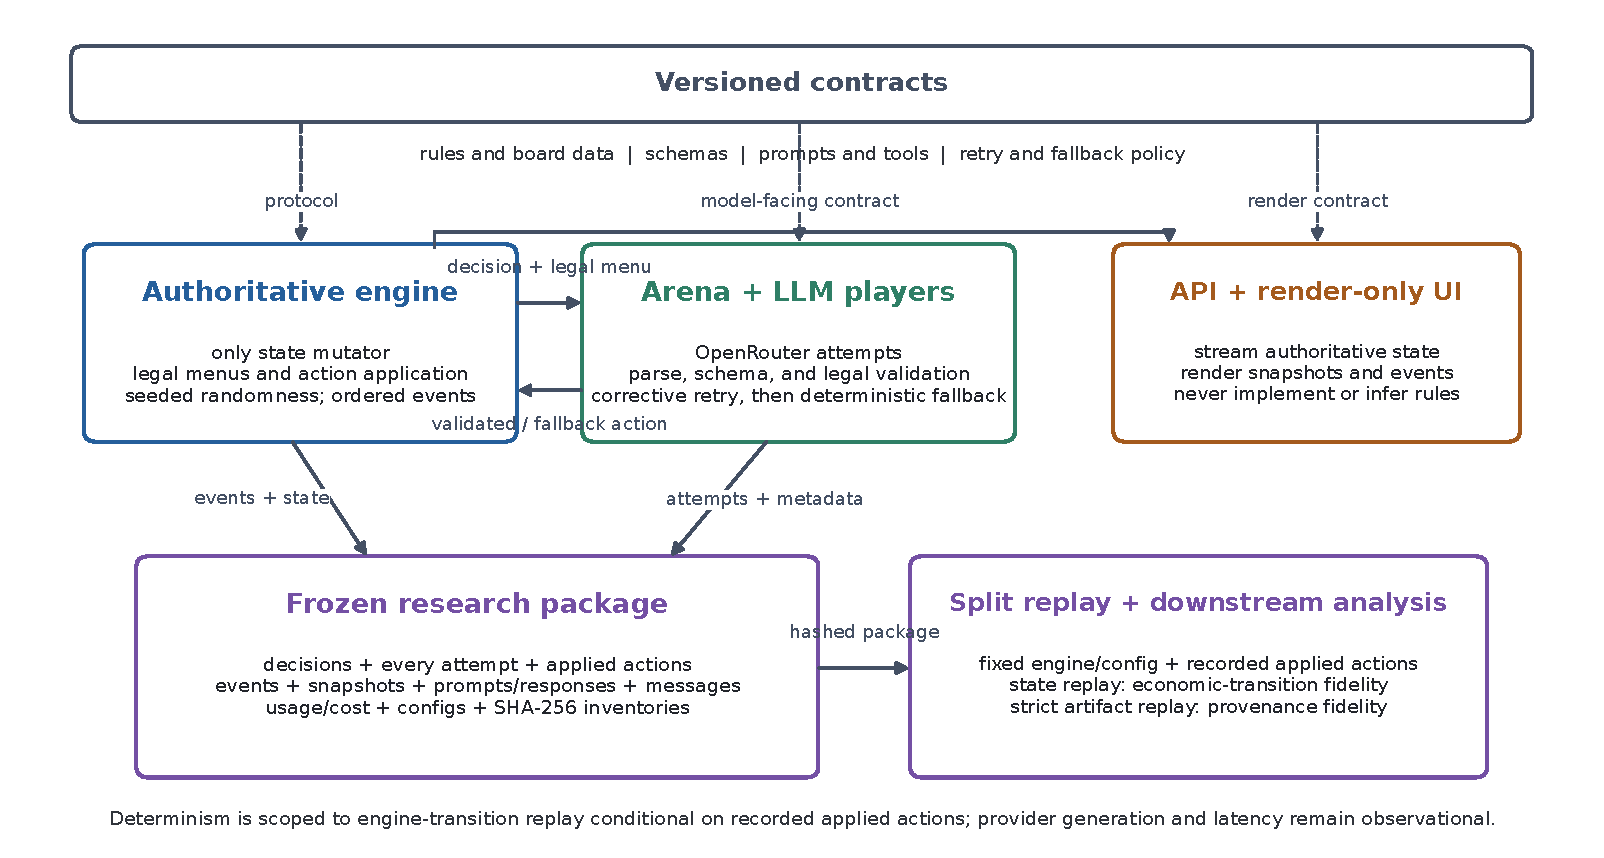
\includegraphics[width=\textwidth]{architecture.pdf}
    \caption{Authority and evidence boundaries. The engine alone mutates game
    state. The arena obtains model selections, validates them against the
    engine-issued menu, retries once when configured, and otherwise applies a
    deterministic fallback. Engine and arena records are frozen and hashed
    together. Replay re-executes the recorded applied-action sequence; it does
    not re-query providers. The live API/UI path renders authoritative server
    state and is separate from the frozen research-package path.}
    \label{fig:architecture}
\end{figure*}

\subsection{Environment and Authority Boundary}

\Bench\ is a four-player, turn-based environment implementing a declared
Monopoly ruleset, including seeded movement and card draws, property
acquisition, open auctions, bilateral trades, color-group development, rent,
jail, mortgages, legal liquidation, and bankruptcy. A game ends when one
player remains solvent or when a configured cap is reached. In a
bankruptcy-terminated game, the final solvent player is the winner. Players
still active at a cap are right-censored in bankruptcy-time analyses; any
cap-based placement or terminal-wealth rule must be declared separately.
The external rules reference is the booklet's classic-rules section, not its
Speed Die variant \cite{hasbro_rules}; when the configured treatment differs
from informal play, the versioned engine contract remains authoritative.

The rules engine is the sole authority over state. It generates legal menus,
validates and applies structured actions, advances the seeded random process,
and emits append-only ordered events. Language-model agents cannot mutate
state and may select only from the menu for the current decision. The arena
constructs model requests and handles parsing, validation, the configured
corrective retry, and deterministic fallback. OpenRouter is the model gateway
\cite{openrouter_docs}. Telemetry records protocol objects and provider
metadata. The API
streams server state, and the frontend renders it without implementing game
rules or inferring legality (Fig.~\ref{fig:architecture}).

\subsection{Decision Loop and Protocol Objects}
\label{sec:decision_loop}

For decision $d$, the engine emits a structured set of legal actions $A_d$ for
one acting player. The arena serializes the configured model-visible state,
scoped history, communication fields, and schemas. An attempt is accepted only
if it parses, satisfies the tool schema, and matches $A_d$. If the first
attempt is invalid, the arena issues the configured corrective retry. If no
valid selection is recovered, a deterministic fallback chooses from $A_d$.
Exactly one action is then applied, and the engine emits its events.

Four stable objects form the replay and explanation boundary:
\begin{itemize}
    \item a \emph{snapshot} is an authoritative serialized checkpoint;
    \item an \emph{event} is an ordered transition or major marker with
    sequence and turn metadata;
    \item a \emph{decision} records the acting player, legal surface,
    attempts, validation outcomes, and resolution; and
    \item an \emph{action} is the single structured move applied for that
    decision.
\end{itemize}
Corrective retries add attempts but not decisions or actions. Telemetry joins
each decision to every attempt, the applied action, emitted event range,
snapshots, prompt and response artifacts, public message, model-authored
private analysis field, usage and cost when reported, latency, and fallback
provenance.
This distinction is
necessary because an invalid attempt may have no state effect, while a
fallback may have a large economic effect.

\subsection{Frozen Artifacts and Split Replay}
\label{sec:replay}

Each saved game is self-contained. Its frozen \texttt{run/} tree includes
ordered events, actions, decisions and attempts, prompt/response artifacts,
snapshots, configuration, provider usage/cost, scorecards, and replay reports.
The accompanying \texttt{quality\_check/} tree records human-readable source
checks. File inventories, byte counts, tree hashes, and SHA-256 digests freeze
the source. A downstream \texttt{analysis/} tree contains deterministic
tables and plots, reconciliation reports, episode reconstructions,
evidence-indexed qualitative review, and generated-output manifests. Derived
analysis may be regenerated; frozen source trees are never rewritten.

Replay uses recorded applied actions rather than new model calls. Given a fixed
compatible engine and contract implementation plus the recorded engine seed,
settings, player identities, and applied-action sequence, the verifier
reconstructs the event trajectory.
\emph{State replay} compares canonicalized state-relevant events.
\emph{Strict artifact replay} compares the complete event stream after the
verifier's versioned canonicalization, including observational communication
and fallback-provenance events. Here ``strict'' denotes equality of that full
canonical event stream; it is distinct from byte-for-byte identity of stored
package files. The two statuses are preserved independently, so a run can be
\texttt{state\_passed\_artifact\_failed}. Provider sampling, routing, endpoint
updates, network timing, and latency remain observational and are not claimed
to be deterministic.

This distinction is material for run
\runid{mock-83265-81ed4937}. State replay matches all 1,640 state-relevant
events. Strict artifact replay compares 3,972 events and differs at two
fallback-response events. The first is sequence 669, event
\runid{evt-000669}, decision \runid{dec-000096}: the original preserves the
fallback-applied \texttt{reject\_trade} as \texttt{valid=false} with
\texttt{error=fallback:illogical\_after\_retry}. The second is sequence 1202,
event \runid{evt-001202}, decision \runid{dec-000186}: the original preserves
\texttt{drop\_out} with
\texttt{error=fallback:malformed\_after\_retry}. Replay reconstructs both
already-applied fallback actions as valid with no error. There are no missing
or extra actions, the decision identifiers reconcile, and state replay passes.
We therefore use this run for state-valid trajectory claims while excluding it
from claims requiring full canonical event-stream identity.

\section{Evaluation Methodology and Corpus}
\label{sec:evaluation}

\subsection{Evidence Layers and Claim Gates}

We organize evidence into four layers (Table~\ref{tab:evidence_layers}).
Observed artifacts establish what the engine exposed and applied.
Deterministic metrics summarize those artifacts under versioned definitions.
Bounded counterfactuals evaluate only declared alternatives and horizons.
Qualitative interpretation connects events into a mechanism while retaining
uncertainty and source IDs. No hidden scalar is treated as a universal
Monopoly strategy oracle.

\begin{table}[t]
\caption{Evidence layers and claim gates.}
\label{tab:evidence_layers}
\centering
\small
\setlength{\tabcolsep}{3.2pt}
\begin{tabularx}{\columnwidth}{p{0.18\columnwidth}YY}
\toprule
\textbf{Layer} & \textbf{Supports} & \textbf{Does not support} \\
\midrule
Observed & Legal menus, actions, events, state, attempts, reported usage/cost &
Unobserved continuations or intent \\
Derived & Versioned accounting, episode, reliability, and trajectory
measures & Universal strategic value \\
Bounded counterfactual & One-step solvency or declared branch/horizon &
Eventual survival or victory without a continuation model \\
Qualitative & Evidence-linked mechanisms and review candidates &
Prevalence, causality, or stable model traits \\
\bottomrule
\end{tabularx}
\end{table}

The present paper reports canonical observations, deterministic derived
metrics, and evidence-linked qualitative cases. Its only counterfactual
statements are one-step accounting claims about actions present in frozen legal
menus; it reports no simulated continuation, welfare estimate, strategic
regret, or counterfactual trade surplus.

A state-valid named episode can support ``in this run'' mechanism language.
Population or ranking claims additionally require preregistered balanced
seed-seat blocks, fixed treatment contracts, game-level uncertainty, and
multiplicity control. High-risk communication labels require evidence for the
exact proposition, its truth status at utterance time, a plausible benefit,
benign alternatives, reviewer confidence, and independent adjudication. A
mutually beneficial trade does not by itself establish collusion, and
public--private divergence alone does not establish deception.

\subsection{Metric Definitions}
\label{sec:metrics}

Longitudinal quantities use authoritative state checkpoints rather than raw
internal event counts. For descriptive plots, we use a versioned face-value
asset-balance proxy
\begin{equation}
W^{\mathrm{face}}_{i,t}
= C_{i,t}+P^{\mathrm{face}}_{i,t}+B^{\mathrm{cost}}_{i,t}
-M^{\mathrm{principal}}_{i,t},
\label{eq:face_wealth}
\end{equation}
where $C$ is cash, $P^{\mathrm{face}}$ is the printed price of currently owned
deeds, $B^{\mathrm{cost}}$ is the current installed building stock valued at
printed construction cost (a hotel is five house-cost units), and
$M^{\mathrm{principal}}$ is the mortgage-principal proxy. This accounting
proxy is not liquidation value, market value, continuation value, or expected
discounted rent. We report cash, productive development, mortgages, and
realized rent separately. Net rent is rent received minus rent paid.

Reliability uses decisions as the main denominator. First-attempt validity is
the fraction of model-required decisions whose initial attempt parses,
validates, and matches the legal menu. Retry recovery conditions on an
invalid first attempt. Fallback rate is fallback-resolved decisions divided
by model-required decisions. Invalid-attempt rate instead uses all attempts as
its denominator. Negotiation metrics use complete proposal-to-resolution
episodes; counters remain in the same episode. Proposal count, acceptance,
transferred assets, retained
liquidity, development, and downstream rent are separate quantities.

Recorded token fields retain provider semantics, and reasoning tokens are not
added again when they are already a subset of output tokens
\cite{openrouter_docs}. Missing usage remains missing rather than being
imputed as zero. Recorded cost reflects the OpenRouter/provider charge for the
run's endpoint, route, date, decision mix, and survival exposure; it is not a
model-intrinsic price.

\subsection{Pilot Corpus and Inferential Boundary}

The corpus contains eight selected four-player games, all ending in bankruptcy
before their configured turn cap. Four frontier-roster games use one fixed
Claude--Gemini--Grok--OpenAI seat order, and a fifth uses a single cyclic
rotation of that order. Two mini-roster games use a fixed
OpenAI--Claude--Gemini--Grok order; a third, the longest mini-roster game,
preserves that order but changes the Gemini endpoint. Turn caps are 400, 500,
or 600 turns. Seeds, seats, rosters, model versions, opponent composition,
caps, execution dates, and provider prices are therefore not balanced. For
this selected corpus, the game is the highest-level observational unit;
turns, decisions, attempts, and the four player-level rows within a game are
dependent. In a matched seat-rotation campaign, the seed block---not an
individual game or decision---would be the inferential replication unit.

The frontier endpoints are Claude Opus 4.8, Gemini 3.1 Pro Preview, Grok 4.3,
and OpenAI GPT 5.5. The mini roster uses Claude Haiku 4.5, Grok 4.3, OpenAI
GPT 5.4 Mini, and either Gemini 3.5 Flash (two games) or Gemini 3 Flash Preview
(the 273-turn game). Endpoint names identify the recorded treatment window,
not timeless model families.

We consequently report exact finite-corpus accounting and named cases, with
no confidence intervals, hypothesis tests, win-rate estimates, or model
ranking. A future comparative design should freeze prompt/tool/retry and
routing contracts, assign a fixed four-model roster to predeclared seed
blocks, rotate each model through every seat, randomize execution order, and
analyze uncertainty at the seed-block level, with games nested within blocks.

\section{Audited Pilot Results}
\label{sec:results}

\subsection{Corpus Accounting, Reliability, and Replay}

Table~\ref{tab:corpus} reconciles every unique decision to one applied action
and every corrective retry to one additional provider attempt. Because the
frozen protocol permits at most one corrective retry per decision, the
difference between 3,790 attempts and 3,696 decisions is exactly 94 retry
attempts. Of the 3,696 decisions, 3,602 were valid on the first attempt
(97.46\%); 88 of the 94 initially invalid decisions recovered on retry, and
six resolved through deterministic fallback. Each fallback decision contains
an invalid initial and invalid corrective attempt, yielding 100 invalid
attempts in total (2.64\% of all attempts). The fallback rate is 0.16\% per
decision. These are accounting ratios for the observed corpus, not estimates
of future endpoint reliability.

\begin{table*}[t]
\caption{Audited eight-game corpus. Run labels encode playable-turn count.
Dec.\ is unique decisions (and, by bijection, applied actions); Att., Ret.,
Inv., and FB are provider attempts, corrective retries, invalid attempts, and
fallback-resolved decisions. Tokens are millions; costs are recorded USD
rounded to two decimals. P and F denote pass and fail. Exact seeds, values, and
full run IDs are preserved in the supplementary claim-source ledger.}
\label{tab:corpus}
\centering
\footnotesize
\setlength{\tabcolsep}{3.3pt}
\begin{tabular}{lrrrrrrrcc}
\toprule
\textbf{Run} & \textbf{Dec.} & \textbf{Att.} & \textbf{Ret.} &
\textbf{Inv.} & \textbf{FB} & \textbf{Tok.} & \textbf{USD} &
\textbf{State} & \textbf{Art.} \\
\midrule
R115 & 366 & 377 & 11 & 13 & 2 & 1.99 & 14.61 & P & P \\
R154 & 396 & 401 &  5 &  5 & 0 & 2.04 &  4.65 & P & P \\
R157 & 346 & 355 &  9 &  9 & 0 & 1.82 &  4.04 & P & P \\
R163 & 364 & 371 &  7 &  7 & 0 & 1.88 & 12.06 & P & P \\
R166 & 488 & 502 & 14 & 14 & 0 & 2.79 & 21.91 & P & P \\
R172 & 613 & 631 & 18 & 20 & 2 & 3.48 & 24.60 & P & P \\
R191 & 583 & 604 & 21 & 23 & 2 & 3.52 & 27.71 & P & F$^\dagger$ \\
R273 & 540 & 549 &  9 &  9 & 0 & 2.95 &  4.24 & P & P \\
\midrule
\textbf{All (1,391 T)} & \textbf{3,696} & \textbf{3,790} &
\textbf{94} & \textbf{100} & \textbf{6} & \textbf{20.47} &
\textbf{113.84} & \textbf{8/8} & \textbf{7/8} \\
\bottomrule
\multicolumn{10}{l}{\footnotesize $^\dagger$~State replay passes; strict
artifact replay has two fallback-provenance mismatches (first: sequence 669).}
\end{tabular}
\end{table*}

The artifact stream records 20,474,750 tokens and \$113.84159595. Usage and
cost are present for 3,789 of 3,790 attempts. The missing record is attempt 0
for decision \runid{mock-83265-81ed4937-dec-000389}, whose preserved provider
payload reports an upstream error; usage and cost remain null rather than
being estimated. Costs are not directly comparable across endpoints because
survival duration, decision type, price, and retry exposure differ.

All eight action sequences pass state replay; seven pass strict artifact
replay. The bounded Run 191 exception is described in
Sec.~\ref{sec:replay}. By contrast, the longest selected game,
\runid{mock-44910-42ec35c5} passes 1,942/1,942 state-event comparisons and
4,102/4,102 strict artifact-event comparisons. Replay health is therefore
reported independently of winner, game length, and strategic interpretation.

\subsection{Cross-Run Descriptive Results}

As a deterministic consistency check, the winner has the largest realized net
rent in each saved trajectory. Net rent accumulates over endogenous survival
duration and is itself part of the bankruptcy mechanism, so this finite-corpus
pattern is not treated as an independent predictor, effect estimate, or
model-comparison result. Exact run-level values are provided in the
supplementary claim-source ledger.

Negotiation volume supplies a useful counterexample. The player sending the
most initial trade proposals lost in five of the eight saved games. In four of
those games the winner sent no initial proposal, and in another the winner sent
one.
Proposal generation therefore measures market activity, not negotiation
quality. Accepted terms, retained liquidity, monopoly completion, productive
development, and downstream rent must be evaluated jointly at the episode
level. Run \runid{mock-2413970733-53b199c1} is the extremal case: GPT initiated
all 133 proposals and all 19 accepted deals, received 13 deeds, transferred 17,
built and later sold eight houses, and reached
\runid{mock-2413970733-53b199c1-dec-000602} with no deed available to
liquidate.

Reliability and economic success are likewise distinct. Some losing players
completed all decisions without an invalid attempt, whereas the winner of Run
115 incurred a fallback. Conversely, serialization failures in Runs 115 and
172 displaced legal actions that would have covered the current payment;
deterministic fallback then selected bankruptcy. Incidence, recovery, fallback
choice, and downstream materiality must therefore be reported separately.

\subsection{Mechanism Case Studies}

Table~\ref{tab:mechanisms} summarizes four source-indexed mechanisms selected
for counterexample value rather than narrative salience. Each row states the strongest
supported boundary. In its source windows, ``d'' and ``e'' abbreviate decision
and event ordinal ranges within the named run; the evidence index resolves
them to complete artifact identifiers.

\begin{table*}[t]
\caption{Mechanism cases. Observations are exact artifact facts; ``immediate
alternative'' means only that an engine-exposed action covered the current
payment; it establishes neither later survival nor victory. Run labels follow
Table~\ref{tab:corpus}.}
\label{tab:mechanisms}
\centering
\small
\setlength{\tabcolsep}{3.4pt}
\begin{tabularx}{\textwidth}{p{0.14\textwidth}p{0.19\textwidth}Yp{0.25\textwidth}}
\toprule
\textbf{Mechanism} & \textbf{Run and source window} &
\textbf{Observed result} & \textbf{Claim boundary} \\
\midrule
Serialization at solvency &
R115: d327--330; e2176--2206 &
A \$197 shortfall; both attempts chose a \$200 sale of eight Brown houses;
malformed calls led to fallback bankruptcy. &
The sale covers the bill with \$3 residual; no continuation result is
established. \\
Blocker exchange &
R157: d251--265, d296--305; e1860--2279 &
Validation blocked an unaffordable bid. Reciprocal swaps completed two groups,
then Orange/Red; the liquid Orange owner built three hotels. &
No oracle establishes fair prices, optimal timing, or a general liquidity
advantage. \\
Creditor transfer &
R163: d120--124, d257--267; e852--875, e1880--1967 &
A \$320 Light Blue purchase became a 3/3/4 build that turn. A later estate
completed the creditor's Red/Green holdings; Red reached 4/4/4. &
One realized seed/seat path; transfers need not yield useful complements. \\
Finite-house coupling &
R273: d395--422, d514--532; e2865--4028 &
A New York exchange preceded nine house purchases and then the final two;
distress-released houses were reacquired. &
Observed scarcity feedback; no branch isolates causality or establishes
optimal retention. \\
\bottomrule
\end{tabularx}
\end{table*}

\paragraph{Reliability can mediate an economic outcome}
In \runid{mock-321229807-87ca99d7}, Claude reached
\runid{dec-000330} with \$1,203 cash against \$1,400 due and eight legally
saleable houses on the Brown group. Both attempts selected the \$200 sale and stated
the correct \$3 residual, but their tool-call shape was invalid. Deterministic
fallback selected bankruptcy and transferred the debtor's cash and six deeds
to Gemini. In \runid{mock-2413970733-53b199c1}, decision
\runid{dec-000582} repeats the pattern: selling one house from each Red
property would
raise \$225 against a \$187 shortfall, but two attempts omitted a required
message field and fallback selected bankruptcy. These cases isolate
serialization from immediate arithmetic; they do not establish the remainder
of either counterfactual game.

\paragraph{Acquisition and productive conversion are distinct}
Run \runid{mock-64394-c3bb8d94} joins auction liquidity, reciprocal exchange,
and development. At \runid{dec-000260}, a \$321 bid for Pacific Avenue was
illegal because the bidder had \$317; validation produced a legal dropout. The
eventual owner of Pacific Avenue then exchanged that deed for Atlantic Avenue
at decisions \runid{dec-000264}--\runid{dec-000265}, completing one color group
for each party. Later, a New York--Kentucky exchange at
\runid{dec-000296}--\runid{dec-000297} completed Orange and Red. The recipient
of the Orange group entered the exchange with substantially more cash and used
\runid{dec-000303}--\runid{dec-000305} to progress from no buildings to three
hotels. Completing a color group did not imply equal conversion speed. Earlier
analysis fields misclassified Kentucky as Orange, showing why
canonical state, legal action, and explanation fidelity must be separated.

\paragraph{Bankruptcy also reallocates productive options}
In \runid{mock-1038910349-f66fa07c}, Claude bought Vermont and Connecticut for
\$320 at decisions \runid{dec-000120}--\runid{dec-000121}, then immediately
developed the Light Blue group to 3/3/4 at
\runid{dec-000122}--\runid{dec-000123}. Much
later, Grok's forced bankruptcy at \runid{dec-000257} transferred seven deeds
and \$295 to the creditor, completing Red and Green. At
\runid{dec-000261}--\runid{dec-000267}, the inherited components were
unmortgaged and the Red group was developed to 4/4/4. The resulting bankruptcy
did more than remove the debtor from play: it transferred strategic
complements and liquidity to the creditor. Bankruptcy to the bank, as in Run
273's terminal tax event, is a counterexample to treating that feedback as
automatic.

\begin{figure*}[t]
    \centering
    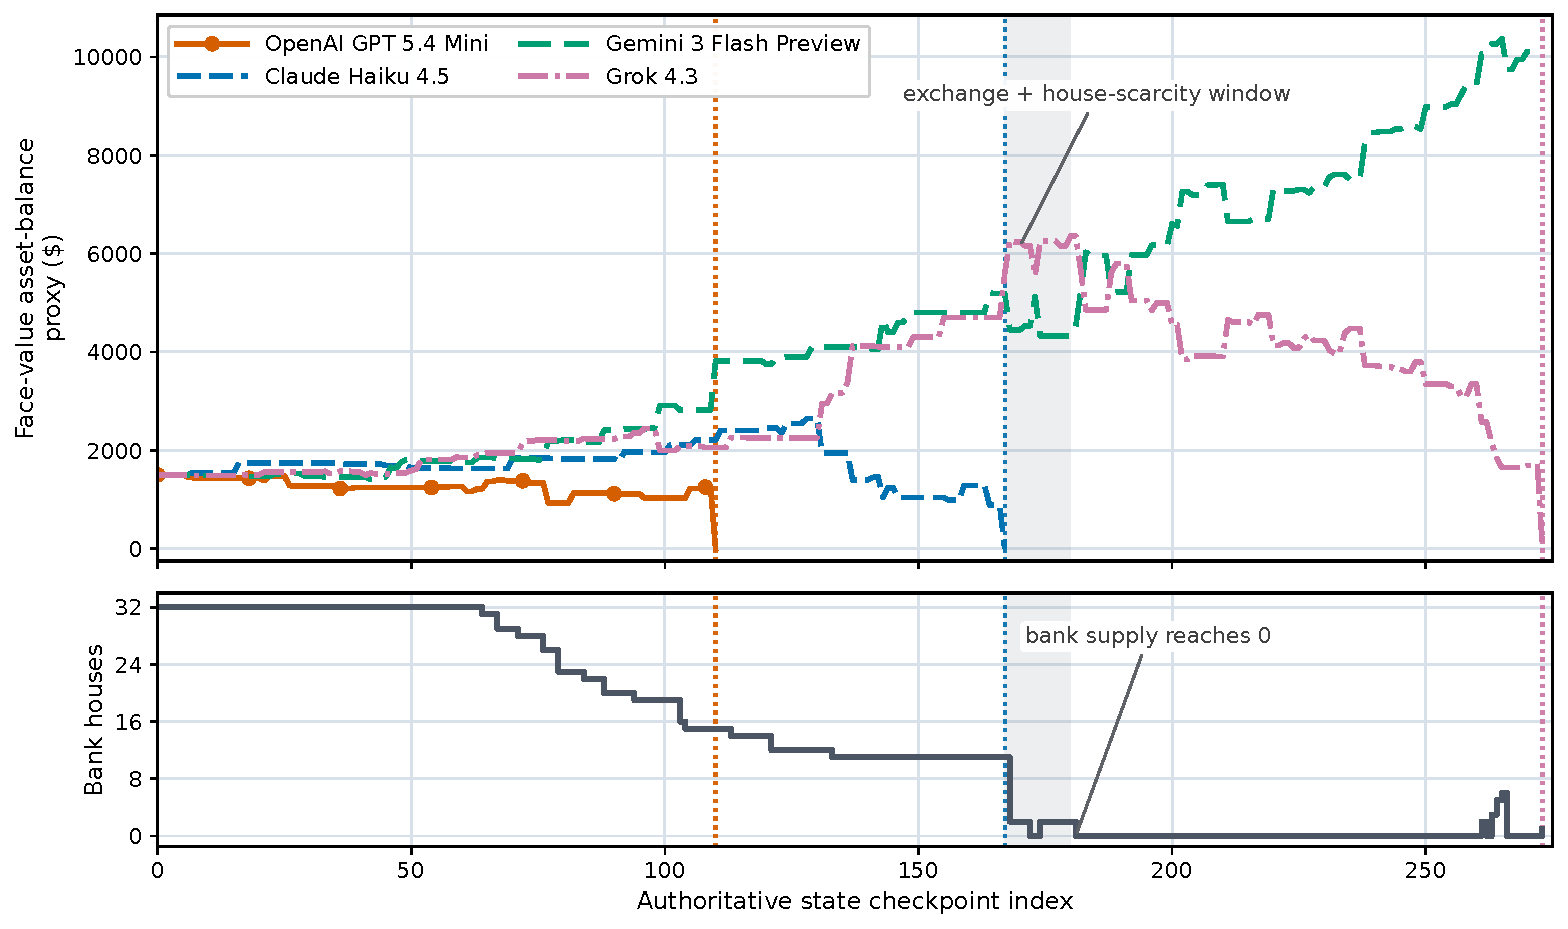
\includegraphics[width=\textwidth]{run273_house_lock.pdf}
    \caption{Run \runid{mock-44910-42ec35c5}. Upper: the face-value
    asset-balance proxy in Eq.~\eqref{eq:face_wealth}; lower: houses remaining in the
    bank. Dotted lines mark the first frozen checkpoints at which GPT, Claude,
    and Grok are bankrupt (110, 167, and 273); their bankruptcy events occur
    on playable turns 109, 166, and 272. The shaded interval covers the
    New York exchange and development sequence at decisions
    \runid{dec-000395}--\runid{dec-000422}. Gemini acquired New York, financed
    nine houses on the Orange group, and then purchased the final two houses in
    the bank. The figure is
    a descriptive trajectory, not a causal estimate of the trade or house
    lock.}
    \label{fig:run273}
\end{figure*}

\paragraph{Finite inventory couples bargaining to later action space}
Figure~\ref{fig:run273} shows the Run 273 mechanism, which passes both replay
checks. Before the
turn-167 exchange, Grok held mortgaged New York while Gemini held the other
Orange deeds and twelve Pink houses; eleven houses remained in the bank.
Gemini offered \$500 plus mortgaged Marvin Gardens and Park Place for New York
at \runid{dec-000395}; Grok accepted at \runid{dec-000396}. Gemini then
mortgaged assets, unmortgaged New York, bought nine houses on the Orange group,
and purchased the final two houses at \runid{dec-000411}. When rent and repairs later forced Grok to
sell Red houses, Gemini reacquired two at \runid{dec-000522} and six at
\runid{dec-000531}. The observed feedback loop is explicit: obligations released a
scarce productive input, and the more liquid player reacquired it. Whether a
different trade, build schedule, or future random path would have been
superior was not evaluated.

\subsection{Communication as Reviewable Evidence}

The artifact contract makes false factual claims, commitments, selective
framing, and ordinary self-interested bargaining separately reviewable against
canonical state and later action; it does not itself adjudicate intent or
deception.

Run \runid{mock-44910-42ec35c5} provides a boundary case. At
\runid{mock-44910-42ec35c5-dec-000395}, Gemini emphasized the counterparty's
Dark Blue completion and liquidity while its model-authored private analysis
field described a plan to consume the remaining houses after receiving New
York. The public proposition was not shown false. The source review therefore
retains the episode as a medium-confidence selective-framing candidate, not a
deception finding.

The supplementary review also records a single-reviewer candidate for
strategic misrepresentation in Run \runid{mock-2413970733-53b199c1}: a stated
plan to retain Ventnor was followed by a later sale. Because the label is
unadjudicated and acute liquidity pressure plus an intervening rejection
support a changed-plan alternative, we do not use it as a paper-level
deception result. Neither case supports a prevalence or model-level claim.

\section{Discussion}
\label{sec:discussion}

\subsection{What the Instrument Measures}

The case corpus is most informative when economic agency is decomposed rather
than collapsed into ownership or victory. Acquisition creates options;
completion of a color group permits development; development creates a rent
schedule; opponent landings convert that schedule into cash; and liquidity
determines whether the developed portfolio can be preserved after a shock.
Mortgages, finite inventory, trades, retries, and bankruptcy transfers couple
these stages. Property count, accepted-trade count, and first-attempt validity
are therefore useful components, not standalone measures of strategy.

This decomposition is a measurement model, not an optimal Monopoly policy. A
blocker can deny an opponent, consume liquidity, serve as collateral, or
become productive after exchange. A mortgage can represent unproductive churn
in one episode and necessary financing in another. A trade can preserve
immediate solvency while surrendering long-horizon income. \Bench's
contribution is that each claimed transition can be checked against a legal
menu and state record. It does not assert that a single heuristic resolves
every tradeoff.

\subsection{Reliability Shapes the Realized Execution Path}

Most invalid attempts did not mutate state, and most corrective retries
recovered a valid action. Yet the two solvency cases show that retry and
fallback policy can translate a coherent model-selected action request into a
different applied action.
Fallback incidence alone misses materiality: the Run 115 winner also incurred
a fallback at the next decision, but that fallback merely ended a turn and
development resumed. Reliability should be analyzed per decision with the
initial menu, each attempt, validation class, corrective prompt, applied
action, fallback rule, and event consequence. This preserves the distinction
among strategic failure, serialization failure, provider failure, retry
recovery, and fallback-policy effect.

\subsection{Baseline and Value-Oracle Boundary}

The current corpus is not balanced, so we do not use a heuristic or learned
Monopoly policy as a performance comparator. Prior Markov and
reinforcement-learning work provides candidate reference policies and state
representations for future work
\cite{monopoly_markov,monopoly_rl,monopoly_drl}, but an unvalidated scalar value
function would overstate what is known about the future course of a negotiated
multi-agent game. The absence of a strategic value oracle limits optimality
and regret claims; it does not prevent assessment of canonical integrity,
reliability accounting, or realized-path mechanisms.

\subsection{From Mechanism Corpus to Comparative Study}

The current result is that the instrument exposes auditable interactions
among acquisition, conversion, negotiation, liquidity, scarce inputs,
reliability, and bankruptcy. The eight trajectories also supply
counterexamples to simple metrics: the most active trade proposer lost in five
of eight games; legal validity did not determine realized economic outcomes;
low cash could coexist with productive assets; and an artifact-provenance
failure did not imply state divergence. These findings motivate hypotheses,
not a leaderboard.

A balanced comparative campaign would require fixed model and routing
treatments, repeated seed blocks, complete seat rotation, randomized execution
order, declared handling of failed runs, and seed-block-level uncertainty.
Capped players would be right-censored for bankruptcy-time analyses. Such a
campaign would answer a different question from the present paper, which
establishes the instrument, artifact contract, and mechanism-level evidence
surface.

\section{Limitations, Ethics, and Reproducibility}
\label{sec:limitations}

\subsection{Limitations}

\paragraph{Selected, dependent observations}
Eight unbalanced games cannot identify provider effects, model rankings, or
mechanism prevalence. Seats and models interact; decisions and turns within a
game are not independent replications. The rent and negotiation observations
are exact descriptions of the saved corpus only.

\paragraph{Realized paths do not identify causal effects}
The artifacts establish what happened under the recorded action sequence.
They do not establish what would follow a different trade, message, build, or
mortgage, because dice, cards, opponents, and later model outputs would
change. We use ``immediate alternative'' only when an engine-exposed action covers
the current payment by exact accounting. This does not imply later survival
or victory.

\paragraph{No universal value oracle}
The face-value asset-balance proxy in Eq.~\eqref{eq:face_wealth} does not value blocker
control, house supply, future landings, bargaining alternatives, or
liquidation friction. Episode rates also depend on denominators, and provider
token semantics differ. We therefore report components, definitions, and
source windows rather than a composite strategic score.

\paragraph{Qualitative labels are not adjudicated traits}
The review packets are evidence-indexed but were produced through a single
review workflow. Model-authored private analysis fields are reports, not direct
access to cognition or intent. Candidate deception, collusion, selective
framing, and ontology-error labels require independent adjudication before any
prevalence or model-level claim.

\paragraph{Stylized domain and implementation scope}
Monopoly is a closed, artificial asset-and-solvency game, not a model of real
firms, finance, welfare, or human economic competence. The declared
\Bench\ ruleset and endpoint policy, rather than informal recollection of
``standard Monopoly,'' define the treatment. External validity is limited to
long-horizon agency under those controlled mechanics.

\subsection{Ethics and Broader Impacts}

This fictional benchmark studies competitive bargaining, strategic
withholding, and public--private divergence and contains no human participants.
Strong labels can anthropomorphize outputs or invite unsupported reputational
claims. We therefore separate factual propositions from model-authored private
analysis fields, retain alternative explanations, and do not treat ordinary
exchange or anti-leader language as deception or collusion. Traces can diagnose
state misrepresentation, solvency errors, interface ambiguity, and harmful
coordination; manipulation analysis is dual-use, so releases should strip
sensitive metadata and frame reviewed tactics as detection evidence.

The corpus consumed 20.47 million recorded tokens and \$113.84 in provider
cost, including retry and failed-attempt overhead where usage was reported;
one provider-error attempt has null usage and cost. Future campaigns should
preregister precision targets and report token use, monetary cost, latency,
and energy use when available.

\subsection{Reproducibility and Artifact Availability}

For each frozen package, we verified deterministic engine-transition
reconstruction with a fixed compatible engine/contract implementation and the
recorded seed, settings, player identities, and applied actions; several legacy
packages omit a run-time engine commit or ruleset hash. Replay does not claim
deterministic regeneration of model selections. Manifests record OpenRouter
reasoning effort \texttt{medium} and no explicit temperature, output-token, or
reasoning-token budget. Routing and reasoning-token semantics remain versioned
provider metadata, not equivalent controls across endpoints
\cite{openrouter_docs}.

The frozen packages preserve linked decisions, attempts, actions, events,
checkpoints, prompts/responses, communication, reported usage/cost, and
configurations. The anonymous review supplement provides the corpus ledger,
claim-source audit, source hashes, replay and coverage reports, evidence
indices, and figures. Manifest-listed ZIP outputs are checked byte-for-byte;
transient cache files are outside that contract. Run
\runid{mock-83265-81ed4937} remains explicitly
\texttt{state\_passed\_artifact\_failed}; its two bounded
fallback-provenance discrepancies at sequences 669 and 1202 are not rewritten
away.

Monopoly is a trademark of Hasbro. \Bench\ is an independent research
implementation and does not imply endorsement.

\section{Conclusion}
\label{sec:conclusion}

\Bench\ turns a long-horizon multi-agent economic game into an auditable
measurement surface. Engine-issued legal actions separate rule enforcement
from strategy, while linked artifacts and split replay expose realized
mechanisms. All eight action sequences reproduce their state trajectories;
seven also reproduce the full canonical event stream, and the remaining run
retains two bounded provenance mismatches. The contribution is the instrument:
a reproducible way to distinguish provider attempts, applied actions, economic
transitions, communication evidence, and artifact integrity without converting
selected games into a model ranking.

\begin{thebibliography}{99}

\bibitem{agentbench}
X. Liu, H. Yu, H. Zhang, Y. Xu, X. Lei, H. Lai, Y. Gu, H. Ding, K. Men,
K. Yang, S. Zhang, X. Deng, A. Zeng, Z. Du, C. Zhang, S. Shen, T. Zhang,
Y. Su, H. Sun, M. Huang, Y. Dong, and J. Tang, ``AgentBench: Evaluating LLMs
as agents,'' in \emph{Proc. Int. Conf. Learn. Representations (ICLR)}, 2024.

\bibitem{taubench}
S. Yao, N. Shinn, P. Razavi, and K. Narasimhan, ``$\tau$-bench: A benchmark
for tool-agent-user interaction in real-world domains,'' in \emph{Proc. Int.
Conf. Learn. Representations (ICLR)}, 2025.

\bibitem{vendingbench}
A. Backlund and L. Petersson, ``Vending-Bench: A benchmark for long-term
coherence of autonomous agents,'' arXiv preprint arXiv:2502.15840, 2025.

\bibitem{dsgbench}
W. Tang, Y. Zhou, K. Cheng, E. Xu, L. Xiao, and M. Li, ``DSGBench: A diverse
strategic game benchmark for evaluating LLM-based agents in complex
decision-making environments,'' in \emph{Proc. IEEE Int. Conf. Acoust.,
Speech Signal Process. (ICASSP)}, Barcelona, Spain, 2026,
pp. 16987--16991, doi: 10.1109/ICASSP55912.2026.11460704.

\bibitem{cattletrade}
R. M\"uller and C. M\"uller, ``Cattle Trade: A multi-agent benchmark for LLM
bluffing, bidding, and bargaining,'' arXiv preprint arXiv:2605.14537, 2026.

\bibitem{monopoly_markov}
R. B. Ash and R. L. Bishop, ``Monopoly as a Markov process,''
\emph{Math. Mag.}, vol. 45, no. 1, pp. 26--29, 1972,
doi: 10.1080/0025570X.1972.11976187.

\bibitem{monopoly_rl}
E. Arun, H. Rajesh, D. Chakrabarti, H. Cherala, and K. George, ``Monopoly
using reinforcement learning,'' in \emph{Proc. TENCON 2019--2019 IEEE Region
10 Conf.}, Kochi, India, 2019, pp. 858--862,
doi: 10.1109/TENCON.2019.8929523.

\bibitem{monopoly_drl}
T. Bonjour, M. Haliem, A. Alsalem, S. Thomas, H. Li, V. Aggarwal,
M. Kejriwal, and B. Bhargava, ``Decision making in Monopoly using a hybrid
deep reinforcement learning approach,'' \emph{IEEE Trans. Emerg. Topics
Comput. Intell.}, vol. 6, no. 6, pp. 1335--1344, Dec. 2022,
doi: 10.1109/TETCI.2022.3166555.

\bibitem{toolprmbench}
D. Li, Y. Yao, Z. Tan, H. Liu, and R. Guo, ``ToolPRMBench: Evaluating and
advancing process reward models for tool-using agents,'' arXiv preprint
arXiv:2601.12294, 2026.

\bibitem{agentrewardbench}
X. H. L\`u, A. Kazemnejad, N. Meade, A. Patel, D. Shin, A. Zambrano,
K. Sta\'nczak, P. Shaw, C. J. Pal, and S. Reddy, ``AgentRewardBench:
Evaluating automatic evaluations of web agent trajectories,'' arXiv preprint
arXiv:2504.08942, 2025.

\bibitem{coffeebench}
I. Sugiura, D. Hattori, K. Araragi, K. Ogawa, S. Onose, T. Makino,
T. Usuki, and T. Ishida, ``CoffeeBench: Benchmarking long-horizon LLM agents
in heterogeneous multi-agent economies,'' arXiv preprint arXiv:2606.16613,
2026.

\bibitem{gamabench}
J.-T. Huang, E. J. Li, M. H. Lam, T. Liang, W. Wang, Y. Yuan,
W. Jiao, X. Wang, Z. Tu, and M. R. Lyu, ``Competing large language models in
multi-agent gaming environments,'' in \emph{Proc. Int. Conf. Learn.
Representations (ICLR)}, 2025.

\bibitem{cicero}
Meta Fundamental AI Research Diplomacy Team (FAIR) \emph{et al.},
``Human-level play in the game of Diplomacy by combining language models with
strategic reasoning,'' \emph{Science}, vol. 378, no. 6624, pp. 1067--1074,
Dec. 2022, doi: 10.1126/science.ade9097.

\bibitem{m3bench}
S. Xie, Z. Shi, H. Shen, Y. Ma, and X. Jing, ``M3-BENCH:
Process-aware evaluation of LLM agents' social behaviors in mixed-motive
games,'' arXiv preprint arXiv:2601.08462, 2026.

\bibitem{sotopia}
X. Zhou, H. Zhu, L. Mathur, R. Zhang, H. Yu, Z. Qi, L.-P. Morency, Y. Bisk,
D. Fried, G. Neubig, and M. Sap, ``SOTOPIA: Interactive evaluation for social
intelligence in language agents,'' in \emph{Proc. Int. Conf. Learn.
Representations (ICLR)}, 2024.

\bibitem{bargaining}
T. Xia, Z. He, T. Ren, Y. Miao, Z. Zhang, Y. Yang, and R. Wang, ``Measuring
bargaining abilities of LLMs: A benchmark and a buyer-enhancement method,''
in \emph{Findings Assoc. Comput. Linguistics: ACL 2024}, Bangkok, Thailand,
2024, pp. 3579--3602, doi: 10.18653/v1/2024.findings-acl.213.

\bibitem{stakeholder}
S. Abdelnabi, A. Gomaa, S. Sivaprasad, L. Sch\"onherr, and M. Fritz,
``Cooperation, competition, and maliciousness: LLM-stakeholders interactive
negotiation,'' in \emph{Advances in Neural Information Processing Systems},
vol. 37, pp. 83548--83599, 2024, doi: 10.52202/079017-2658.

\bibitem{agenticpay}
X. Liu, S. Gu, and D. Song, ``AgenticPay: A multi-agent LLM negotiation
system for buyer-seller transactions,'' arXiv preprint arXiv:2602.06008,
2026.

\bibitem{hasbro_rules}
Hasbro, ``Monopoly: Property trading game from Parker Brothers,'' rules
booklet no. 00009-1, 2007. [Online]. Available:
\url{https://www.hasbro.com/common/instruct/00009.pdf}. Accessed:
Jul. 28, 2026.

\bibitem{openrouter_docs}
OpenRouter, ``Reasoning tokens; API parameters; Provider routing,'' official
documentation, accessed Jul. 28, 2026. [Online]. Available:
\url{https://openrouter.ai/docs/guides/best-practices/reasoning-tokens};
\url{https://openrouter.ai/docs/api_reference/parameters};
\url{https://openrouter.ai/docs/guides/routing/provider-selection}

\end{thebibliography}

\end{document}
